\section{Analyse eines optimalen DevSecOps Prozesses}\label{sec:analysisDevSecOps}
Was ist DevSecOps?
Warum benötigt man DevSecOps?
Wie sollte DevSecOps aussehen?
Was muss man beachten?

Diese Fragen sollen in der folgenden Analyse Schritt für Schritt beantwortet werden und bilden die Basis für das grundlegende Verständnis von DevSecOps Prozessen.

\subsection{DevOps}
Die Frage, was DevOps eigentlich sei, ist etymologisch schnell beantwortet.
DevOps ist ein Kofferwort aus den Komponenten "Development" und "Operations".
Die Bedeutung dieses Begriffs hingegen stellt sich als weit weniger eindeutig heraus.
Die Antwort auf die Frage nach der Bedeutung ist vielmehr ein Verständnis für ein Ziel, welches versucht wird zu erreichen, eine Philosophie Prozesse zu optimieren und ein "Ansatz, wie die Zusammenarbeit zwischen Softwareentwicklung und IT-Betrieb verbessert werden kann."\cite{DevOps2021}

Microsoft Azure, einer der führenden Betreiber im DevOps Segment, beschreibt in einem Blogpost diese Philosophie als eine Art Brücke zwischen IT-Betrieb, Qualitätstechnik und Sicherheit\cite{WasIstDevOps}:
\begin{quote}
    DevOps ermöglicht es zuvor getrennten Rollen wie Entwicklung, IT-Betrieb, Qualitätstechnik und Sicherheit, sich zu koordinieren und zusammenarbeiten, um bessere und zuverlässigere Produkte zu liefern. Durch die Einführung der DevOps-Kultur mit DevOps-Methoden und -Tools können Teams besser auf die Anforderungen ihrer Kunden reagieren, das Vertrauen in ihre eigenen Anwendungen steigern und Geschäftsziele schneller erreichen.
\end{quote}

Zusammenfassend lässt sich sagen, dass DevOps ein Mindset, eine Philosophie oder ein Prozess ist, der den von Natur aus zyklischen Prozess der Softwareentwicklung automatisieren, koordinieren und beschleunigen soll.
Was zunächst komplex klingt kann heutzutage mithilfe vieler Tools auf dem Markt verhältnismäßig leicht erreicht werden.
Im Laufe des Seminars wurde hierfür primär die Plattform GitLab CI eingesetzt, welche auch hier später als Beispiel dienen wird.
Wichtig ist allerdings ein Verständnis dafür zu entwickeln, dass GitLab nicht die Lösung für DevOps ist, sondern nur ein Tool, wie viele andere auch, um das Mindset eines Entwickler- und Operationsteams elegant umsetzen zu können.

\subsection{Left Shift in DevOps}

Der Begriff "Left Shift" beschreibt den Ansatz Tests so früh wie möglich, also weiter \textit{links} auf einem virtuellen Zeitstrahl, zu machen.
Dadurch entsteht ein erhöhter Fokus auf dem Testen und somit im Idealfall auch eine höhere Qualität in der Software.\cite{dr.darrellr.schragDevOpsShiftLeft2016}
Dies geschieht durch das direkte Feedback, welches nun an jeden commit geknüpft ist.
Somit können Unschönheiten und Fehler direkt behoben werden, ohne dass sie weitere negative Effekte auslösen können.

Dies muss sich nicht ausschließlich auf Unit-/Integration- und End-To-End-Tests beziehen, sondern kann auch auf Security Tests, hier im Speziellen \hyperref[subsubsec:dast]{DAST}, bezogen werden.
Hierbei kann man sogar so weit gehen, dass alle sicherheitsrelevanten Tests nach jedem Commit ausgeführt werden sollten, selbst wenn diese eine hohe Zeit in Anspruch nehmen.
Dies hat den Vorteil, dass Entwickler ein umgehendes Feedback erhalten, über alle Sicherheitslücken, die in dem aktuellen Commit gefunden werden.
Daher wird dies auch von vielen Experten empfohlen, unter welchen auch GitLab ist, deren Tool die Grundlage für die Umsetzung einer Pipeline in diesem Seminar geboten hat.\cite{gitlabSeismicShiftApplication2020}
Dadurch, dass Sicherheitslücken nun gemeinsam mit den Testergebnissen direkt an die Entwickler zurückgegeben werden fließt das Beheben von Sicherheitslücken nahtlos in den Prozess der Behebung von Fehlern und der Entwicklung neuer Features ein.


\subsection{DevSecOps}

Etymologisch lässt sich auch der Begriff DevSecOps schnell erklären.
Das Kofferwort DevOps wurde lediglich um die Komponente der "Security" erweitert.
In der Umsetzung ist dies allerdings nicht so einfach, wie es auf den ersten Blick scheint.
IT-Sicherheit ist grundsätzlich ein Wettrennen.
Während einige Entwickler/Security Experten versuchen eine Software zu schützen, versuchen Hacker Schwachstellen zu finden und zu nutzen.
Außerdem ist IT-Sicherheit ein sehr komplexes Thema, welches in nahezu jedem Fall Experten benötigt.
Allerdings lassen sich auch viele Teile der Überprüfung auf Schwachstellen automatisieren und nach links shiften.

\subsection{Entwicklungsprinzipien}

Kanban, Scrum, Waterfall oder etwas Eigenes erfinden?
Der Bereich der agilen Entwicklung hat in den letzten Jahren viele verschiedene Verfahren entwickelt, um Projekte zu managen und agil zu arbeiten.
"Agile Softwareentwicklung zeichnet sich durch selbstorganisierende Teams sowie eine iterative und inkrementelle Vorgehensweise aus."\cite{AgileSoftwareentwicklung2021}
Der Kern agiler Softwareentwicklung ist also, das Kurzhalten von Planungsphasen und damit einhergehender kontinuierlicher weiterer Planung zur Laufzeit des Projekts.
Ähnlich wie bei DevOps ist das Ziel, sich möglichst schnell und flexibel auf Änderungen anpassen zu können, kontinuierlich neuen Code vorweisen können und sich "in regelmäßigen, kurzen Abständen mit dem Kunden [abstimmen]"\cite{AgileSoftwareentwicklung2021} zu können und dabei die Codequalität zusätzlich positiv zu beeinflussen.
Hier greifen DevOps und agile Methoden natürlich Hand in Hand.
Agile Methoden können sehr schnell sehr viele Aspekte mit sich bringen und sind als eigenes Thema in einer Arbeit sicher besser aufgehoben.
Dennoch soll hier ein grundlegendes Verständnis für Kanban, Scrum und Waterfall gegeben werden, da agile Entwicklung eine wichtige Voraussetzung für ein gutes und erfolgreiches DevOps orientiertes Projekt ist.

\subsubsection{Kanban}\label{subsubsec:kanban}

Wie bei vielen agilen Methoden steht im Zentrum von Kanban ein Board für die visualisierung einzelner Arbeitsschritte.
Auf diesem sind alle zu tätigen Aufgaben eingetragen, welche Schritt für Schritt in Bearbeitung gehen können.
Zur Unterscheidung dieser Zustände führt man mehrere, aber mindestens drei, Spalten ein.
Diese sind meist mit den Begriffen "Backlog", "In Progress" und "Completed" gekennzeichnet.
Im Backlog befinden sich alle noch nicht begonnenen Aufgaben, die bei Bedarf in Bearbeitung gehen können.
In diesem Fall wird die Karte aus der Spalte "Backlog" in die Spalte "In Progress" bewegt, um für alle Mitarbeitenden zu signalisieren, dass an dieser Aufgabe bereits gearbeitet wird.
Nach Fertigstellung einer dieser Karten wird diese in die Spalte "Completed" verschoben und ist damit erledigt.
Um verschiedene Wichtigkeitsstufen abbilden zu können ist möglich verschiedene sog. Lanes zu verwenden.
Diese werden als einzelne Reihen dargestellt, von denen in der Regel obere Reihen vor unteren Reihen bearbeitet werden sollen.
Zudem limitiert man die Anzahl maximal erlaubter Tickets in Bearbeitung, um zu starkes Multitasking und damit einhergehender sinkender Effizienz zu vermeiden.

Die Vorteile eines solchen Prinzips liegen auf der Hand.
Durch ein sehr offenes, transparentes Prinzip entsteht ein gleichmäßiger Workflow, der sich in den meisten Situationen einfach in bestehende Prozesse integrieren lässt.

Dem entgegen steht die Abwesenheit von Zeitplanung, was Probleme bei der Einhaltung von Deadlines erzeugen kann, sowie die Bedingung Arbeit in einzelne Schritte aufteilen zu können.
Speziell letzteres ist in der Softwareentwicklung zwar meist kein Problem, allerdings dennoch häufiger als Erwartet ein Problem, wenn an großen zusammenhängenden Features gearbeitet werden muss.\cite{Kanban}

\subsubsection{Scrum}

Atlassian, zieht bei der Beschreibung von Scrum eine sehr passende Football Analogie heran\cite{atlassianScrumWasEs}:
\begin{quote}
    Scrum ist ein Framework, das die Zusammenarbeit in Teams unterstützt. \textit{Scrum} steht im Rugby für \textit{Gedränge} – und genau wie ein Rugbyteam, das für das große Spiel trainiert, sind Teams mit Scrum in der Lage, durch Erfahrungen zu lernen, sich bei der Problembehebung selbst zu organisieren sowie ihre Erfolge und Niederlagen zu reflektieren, um sich kontinuierlich zu verbessern.
\end{quote}

Ähnlich wie bei \hyperref[subsubsec:kanban]{Kanban} werden Aufgaben aufgeteilt in "Backlog", "In Progress" und "Completed".
Allerdings liegt ein weitaus größerer Fokus auf der Zeitplanung, die bei Kanban vollständig weg gelassen wird.
Im Gegensatz zu Kanban werden die Aufgaben nicht einfach bearbeitet, sobald die vorherige Aufgabe abgeschlossen wird, sondern es wird für einen kurzen Zeitraum, meist zwei Wochen, geplant, welche Aufgaben zu erledigen sind.
Dieser Zeitraum nennt sich Sprint und stellt die Basis von Kanban dar.

\subsubsection{Waterfall}

\subsubsection{Fazit}

Alle oben genannten Methoden bieten eine gute Grundlage für DevSecOps.
Insgesamt muss jedes Team für sich entscheiden, welches Entwicklungsprinzip für sie am besten funktioniert.
Alle Prinzipien einmal auszuprobieren ist definitiv empfehlenswert, um den optimalen Workflow für sein Team und seine Usecases finden zu können.

\subsection{Git Struktur/Branching}

Bevor eine Betrachtung der einzelnen Schritte im Prozess stattfinden kann, muss zunächst die Grundstruktur des Versionskontrollsystems (VCS) geklärt sein.
In diesem Seminar wurde als VCS GitLab (git) verwendet, weshalb dieses auch hier als Grundlage dienen soll.
Wenn es um das Thema Struktur im git geht, entstehen häufig hitzige Diskussionen unter Entwicklern.
Die Menge an möglichen Modellen ist scheinbar endlos.
In der Vergangenheit hat sich oft gezeigt, dass git-flow\cite{SuccessfulGitBranching} eine gute Möglichkeit ist, um sein git zu ordnen.
Allerdings ist dieses Modell sehr kompliziert, weshalb von diesem Modell heutzutage oftmals abgeraten wird.
Ein häufig vorgeschlagenes Alternativmodell stellt GitHub flow\cite{UnderstandingGitHubFlow} dar.
Dieses Modell ist im Gegensatz zu git-flow sehr einfach gestrickt.
So einfach, dass Testumgebungen nicht wirklich anhand der gegebenen Branches dargestellt werden können.
Deshalb empfiehlt sich die Verwendung eines Modells, das zwischen git-flow und GitHub flow anzuordnen ist.
\begin{figure}[H]
    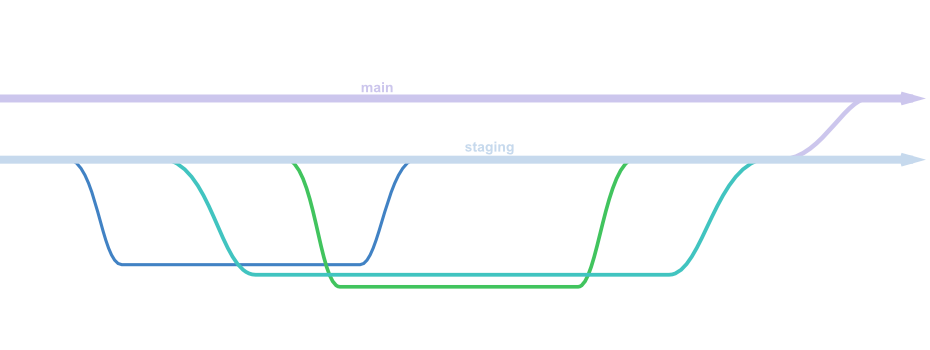
\includegraphics[width=0.8\textwidth]{img/branching}
    \centering
    \caption{Graphische Darstellung der Kombination aus git-flow und GitHub Flow}
    \label{fig:branchingModel}
\end{figure}

Das hier gezeigte Modell basiert relativ stark auf GitHub flow.
Es gibt einen Hauptbranch (Main), welcher zu jeder Zeit veröffentlichbar sein sollte.
Im Gegensatz zu GitHub flow ist dies allerdings nicht der main Branch, sondern ein staging Branch.
Dieser kann dann Nutzern als Beta-Version zur Verfügung gestellt werden.
So haben Nutzer die Möglichkeit neue Features sofort zu testen und direktes Feedback in den Entwicklungsprozess zurück zu bringen.
Im Gegensatz zu GitHub flow ist dies allerdings nicht der Branch, der in Production veröffentlicht wird.
Dafür gibt es den main branch, für den die gleichen Kriterien gelten wie für den Staging Branch.
Zudem darf auf den main branch allerdings nur eine getestete Version vom Staging Branch deployed werden.
Entwicklung sollte allerdings, genau wie bei GitHub flow, auf dem Main und Staging branch nicht stattfinden.
Hierfür werden für jedes Feature eigene Branches aufgemacht (dunkelblau, hellblau und grün in Abbildung~\ref{fig:branchingModel}).
Auf diesen werden alle commits gepushed, bis das feature bereit ist, in den Staging branch gemerged zu werden.
Dies bedeutet, dass das Feature vollständig funktioniert.
Sobald dieses Stadium erreicht ist, wird ein Pull Request in den Staging Branch erstellt.
Hiermit wird der Review Prozess eingeleitet.
Zunächst laufen natürlich alle automatisierten Tests und stellen die Codequalität und -funktionalität bestmöglich fest.
Im nächsten Schritt sollte der Merge Request von anderen Personen bestätigt werden und mögliche Fehler und Unstimmigkeiten sollten behoben werden.
Sobald diese Schritte durchlaufen sind, kann das Feature in den Staging Branch gemerged werden.
Nun rollt die Pipeline das Feature automatisch an alle Beta Nutzer aus, sodass eine realistische Testumgebung Feedback in den Entwicklungsprozess zurückspielen kann.
Unter der Annahme, dass hierbei keine Fehler auftreten kann man nun mit erhöhter Sicherheit und Stabilität den Staging Branch nach einem Pull Request in den Main Branch mergen, was ein Deployemnt für alle Nutzer auslöst.

Die Vorteile gegenüber GitHub flow liegen auf der Hand.
Ein Branchingmodell, welches nur minimal komplizierter ist, bringt eine stark erhöhte Stabilität im Programm, da Features zunächst an eine kleine Testgruppe ausgerollt wird, Feedback gesammelt wird und dieses erneut in den Entwicklungsprozess einfließen kann, bevor ein Feature an alle Nutzer ausgerollt wird.
Alle Vorteile von GitHub Flow gegenüber git-flow bleiben allerdings erhalten, weshalb dies immer noch ein exzellentes Modell für DevOps ist.

\subsection{DevSecOps Pipelines}

Pipelines bilden die Grundlage in der Umsetzung eines erfolgreichen DevSecOps Projekts.
Grundsätzlich lassen sich Pipelines in drei Bereiche unterteilen: Testen, Bauen und Deployen.
Allerdings lassen sich diese Schritte nicht immer einfach nacheinander ausführen, da Schritte im Test zum Beispiel von einem Build oder Deployment abhängen können, genauso wie ein Deployment von einem Test und offensichtlich einem Build abhängen kann.
Daher werden die einzelnen Schritte im Folgenden nacheinander betrachtet und analysiert.
Diese sind chronologisch so angeordnet, wie sie auch im finalen Prozess vorhanden sein sollten.

\subsubsection{Coding Guidelines/Code Architecture}\label{subsec:codingGuidelines/codeArchitecture}

Nachdem nun klar ist, in welcher Struktur der Code im VCS vorzufinden ist, gilt es nun die einzelnen Schritte in der Pipeline zu betrachten.
Hierbei sollte mit den Syntax- und Architekturtests begonnen werden.
Bevor die Funktionalität einer Software getestet wird, sollte immer sichergestellt sein, dass die Architektur und Syntax den gewählten Konventionen entspricht.
Für die Bewertung der Position eines Schrittes in einer Pipeline gibt es mehrere ausschlaggebenden Punkte, welche bei jedem Job in der Pipeline betrachtet werden sollten.
\begin{itemize}
    \item Welche Abhängigkeiten existieren zu anderen Schritten?
    \item Wie hoch ist die Zeitkomplexität des Jobs?
    \item Wann muss dieser Job ausgeführt werden?
\end{itemize}

\paragraph{Welche Abhängigkeiten existieren zu anderen Schritten?}

Bei der Betrachtung der Abhängigkeiten zu anderen Schritten liegt auf der Hand, dass nichts außer dem Source Code nötig ist, um dessen Qualität zu testen.
Somit gibt es keine anderen Jobs, welche vor diesem Job auszuführen sind.
Dies ist auch der Grund, weshalb dieser Schritt zu Beginn der Pipeline angeordnet sein sollte.

Da auch keine anderen Tests Abhängigkeiten zu Architektur- und Syntaxtests haben lassen sich diese auch problemfrei zu anderen Tests parallelisieren.

\paragraph{Wie hoch ist die Zeitkomplexität des Jobs?}

Syntax- und Architekturtests sind in relativ kurzer Zeit auszuführen, da keine externen Abhängigkeiten oder komplexe Build Prozesse nötig sind.
Dies ist speziell in den ersten Jobs äußerst erstrebenswert, da die Pipeline möglichst früh fehlschlagen sollte, wenn Fehler existieren, um unnötige Verzögerungen im Entwicklungsprozess zu vermeiden.
Zudem ist auch die Behebung von Syntaxfehlern zumeist relativ schnell erledigt, sodass zügig die weiteren Schritte der Pipeline erreicht werden können.

\paragraph{Wann muss dieser Job ausgeführt werden?}

Bei dieser Frage ist die Zeitkomplexität oftmals ein großer Faktor.
Tests, die kaum Zeit in Anspruch nehmen kann man ohne große Einschränkungen häufiger ausführen.
Dementsprechend empfiehlt es sich hier, die Tests bei jedem commit auszuführen, um stets eine gute Codequalität gewährleisten zu können und bereits früh im Prozess korrigieren zu können, falls die Architektur nicht den gesetzten Standards entspricht.

\subsubsection{Vulnerability Checker}

Bei der Entwicklung großer Projekte ist es kaum möglich externe Abhängigkeiten zu vermeiden.
Für nahezu jedes Framework und jede Programmiersprache existieren Package Manager, die den Prozess externe Pakete ins Projekt einzufügen extrem vereinfachen.
Diese Leichtigkeit löst allerdings ein Problem aus.
Viele Libraries wurden selbst von unerfahrenen Entwicklern geschrieben, oder wurden in sehr kurzer Zeit entwickelt, was zu Fehlern und vor allem zu Sicherheitslücken führen kann.
Die Entwicklercommunity kann diese zwar häufig relativ schnell finden und identifizieren, aber Maintainer können die Sicherheitslücken oftmals nicht sofort schließen.
Daher ist ein wichtiger Faktor einer guten Pipeline

\paragraph{Welche Abhängigkeiten existieren zu anderen Schritten?}
\paragraph{Wie hoch ist die Zeitkomplexität des Jobs?}
\paragraph{Wann muss dieser Job ausgeführt werden?}

\subsubsection{Test-/Codeabdeckung}
\paragraph{Welche Abhängigkeiten existieren zu anderen Schritten?}
\paragraph{Wie hoch ist die Zeitkomplexität des Jobs?}
\paragraph{Wann muss dieser Job ausgeführt werden?}

\subsubsection{Lizenzüberprüfung}
\paragraph{Welche Abhängigkeiten existieren zu anderen Schritten?}
\paragraph{Wie hoch ist die Zeitkomplexität des Jobs?}
\paragraph{Wann muss dieser Job ausgeführt werden?}

\subsubsection{Repository Manager}
\paragraph{Welche Abhängigkeiten existieren zu anderen Schritten?}
\paragraph{Wie hoch ist die Zeitkomplexität des Jobs?}
\paragraph{Wann muss dieser Job ausgeführt werden?}

\subsubsection{Dynamic Application Security Testing (DAST)}\label{subsubsec:dast}
\paragraph{Welche Abhängigkeiten existieren zu anderen Schritten?}
\paragraph{Wie hoch ist die Zeitkomplexität des Jobs?}
\paragraph{Wann muss dieser Job ausgeführt werden?}

\subsubsection{Code Review}
\paragraph{Welche Abhängigkeiten existieren zu anderen Schritten?}
\paragraph{Wie hoch ist die Zeitkomplexität des Jobs?}
\paragraph{Wann muss dieser Job ausgeführt werden?}

\subsubsection{Application Monitoring}
\paragraph{Welche Abhängigkeiten existieren zu anderen Schritten?}
\paragraph{Wie hoch ist die Zeitkomplexität des Jobs?}
\paragraph{Wann muss dieser Job ausgeführt werden?}
